%\documentstyle[epsf,twocolumn]{jarticle}       %LaTeX2e仕様
%\documentclass[twocolumn]{jarticle}     %pLaTeX2e仕様(platex.exeの場合)
\documentclass[onecolumn]{ujarticle}     %pLaTeX2e仕様(uplatex.exeの場合)
%%%%%%%%%%%%%%%%%%%%%%%%%%%%%%%%%%%%%%%%%%%%%%%%%%%%%%%%%%%%%%
%%
%%  基本バージョン
%%
%%%%%%%%%%%%%%%%%%%%%%%%%%%%%%%%%%%%%%%%%%%%%%%%%%%%%%%%%%%%%%%%
\setlength{\topmargin}{-45pt}
%\setlength{\oddsidemargin}{0cm} 
\setlength{\oddsidemargin}{-7.5mm}
%\setlength{\evensidemargin}{0cm} 
\setlength{\textheight}{24.1cm}
%setlength{\textheight}{25cm} 
\setlength{\textwidth}{17.4cm}
%\setlength{\textwidth}{172mm} 
\setlength{\columnsep}{11mm}

%\kanjiskip=.07zw plus.5pt minus.5pt


% 【節が変わるごとに (1.1)(1.2) … (2.1)(2.2) と数式番号をつけるとき】
%\makeatletter
%\renewcommand{\theequation}{%
%\thesection.\arabic{equation}} %\@addtoreset{equation}{section}
%\makeatother

%\renewcommand{\arraystretch}{0.95} 行間の設定
%%%%%%%%%%%%%%%%%%%%%%%%%%%%%%%%%%%%%%%%%%%%%%%%%%%%%%%%
%\usepackage{graphicx}   %pLaTeX2e仕様(\documentstyle ->\documentclass)
\usepackage[dvipdfmx]{graphicx}
\usepackage{subcaption}
\usepackage{multirow}
%%%%%%%%%%%%%%%%%%%%%%%%%%%%%%%%%%%%%%%%%%%%%%%%%%%%%%%%
\begin{document}
	
	%bibtex用の設定
	%\bibliographystyle{ujarticle} 
	
	\noindent
	
	\hspace{1em}
	2019 年 6 月 28 日
	ゼミ資料
	\hfill
	M1 寺内 光
	
	\vspace{2mm}
	
	\hrule
	
	\begin{center}
		{\Large \bf 進捗報告}
	\end{center}
	
	
	\hrule
	\vspace{3mm}
	
	% ‚ここから 文章 Start!
	\section{レイヤ抜きデータオーギュメンテーションの実装中}
	ある画像が $n$ 枚のレイヤ ($\rm{L}_{1}$, $\rm{L}_{2}$, ..., ${\rm{L}}_{i}$, ... , ${\rm{L}}_{n}$)から構成されているとき,長さ $n$ のバイナリ系列 B を与え,${\rm{B}}_{i}$が 1 のときレイヤ${\rm{L}}_{i}$を採用するというデータオーギュメンテーションを行うジェネレータを作成中である.このオーギュメンテーションによって学習データセットは単純に $2^{n}$ 倍に増やすことができる.
	このジェネレータはセマンティックセグメンテーションを行うクラス, 画像サイズ,バッチサイズを引数にとり,上記の方法で生成した学習画像とそのターゲット画像を返す.ここでターゲット画像はクラスをそれぞれ整数に置き換えたものをピクセルに対応付けて格納した 2 重配列である(サイズは学習画像と同じ).また,ジェネレータとして定義することで keras のモデルで学習できるように設計している.ただし,現在の時点では,“あるレイヤ”が“あるクラス”に属しているかどうかを判断する方法はファイル名との文字列一致によってのみ行われるため,今使えるセマンティックセグメンテーションのクラスは目(と口と眉)のみである.そこでまずは目の領域を識別できるかどうかのタスクをやってみたいと考えている.
	
	上記の機能を少し実装したので実際に生成(yield)されたオーギュメント画像とそれに対応するターゲット画像の一例を図 \ref{fig:data_and_target} に示す.今回はクラスとして口のみを指定したため,ターゲット画像の中身は口の領域のみ 0,それ以外は 1 が入っている.図 \ref{fig:data_and_target} ではわかりやすく 0 が入っている領域を黒くしている. 
	\begin{figure}[h]
		\vspace{-4mm}
		\centering
		\begin{subfigure}{0.49\columnwidth}
			\centering
			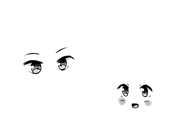
\includegraphics[width=1.2\columnwidth]{data.png}
			\caption{オーギュメントデータ画像}
			\label{fig:data}
		\end{subfigure}
		\begin{subfigure}{0.49\columnwidth}
			\centering
			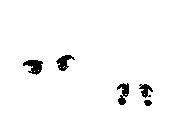
\includegraphics[width=1.2\columnwidth]{target.png}
			\caption{ターゲット画像}
			\label{fig:target}
		\end{subfigure}
		\caption{オーギュメント画像とそのターゲット画像の一例}
		\label{fig:data_and_target}
	\end{figure}

	\section{来週以降のタスク}
	現時点ではレイヤの組み合わせがあまりにも多い(データ数が 1000 倍になると仮定すると 24 万枚の学習をすることになる)のでもう少し妥当な数に調整できるパラメータを追加する.
	また,どのような画像が学習に適当かどうかを上野さんとのミーティングですり合わせる.

\end{document}